
Let $G$ be a group and $\Gamma$ be another group with a left action of $G$.
Then, there is a \emph{semidirect product} group $\Gamma \rtimes G$ whose underlying set is the Cartesian product $\Gamma \times G$ but whose multiplication is twisted by the action:
\[
(\delta, h) \cdot (\gamma, g) = (\delta (h \triangleright \gamma), hg), \qquad \delta, \gamma \in \Gamma, \quad h, g \in G.
\]

Now we consider this constrution w.r.t. coordinate rings.
Let $H = k[G]$ be the coordinate ring of $G$, and $A = k[\Gamma]$ be the coordinate ring of $H$.
The left action of $G$ on $\Gamma$ now turns into the right coaction $\beta: A \rightarrow A \otimes H$ such that
\[
a(h \triangleright \gamma) = a_0(\gamma) a_1(h).
\]
where $\delta(a) = a_0 \otimes a_1$.

The above argument shows that, the coordinate ring of $\Gamma \rtimes G$ is a vector space $H \otimes A$ whose comultiplication is given as
\[
\Delta(f \otimes a) = (f_1 \otimes f_{2,0} a_1) \otimes (f_{2,1} \otimes a_2).
\]

We will denote this coalgebra by $H \ltimes A$.
At first, we consider its algebra version with fewer assumption.

\begin{proposition} \cite[Prop.1.6.6]{Foundation}
    Let $H$ be a bialgebra and $A$ be a left $H$-module algebra.
    There is a \emph{left cross product} algebra $A \rtimes H$ built on $A \otimes H$ with product
    \[
    (a \otimes h)(b \otimes g) = a(h_1 \triangleright b) \otimes h_2 g \quad a,b \in A, \quad h, g \in H.
    \]
    The unit element is $1_A \otimes 1_H$.
\end{proposition}
\begin{proof}
    It is easily to check that $1_A \otimes 1_H$ is a unit:
    \[
    (1_A \otimes 1_H)(b \otimes g) = (1 \triangleright b) \otimes g = b \otimes g, \quad (a \otimes h)(1_A \otimes 1_H) = a(h_1 \triangleright 1_A) \otimes h_2 = a \otimes h.
    \]
    Note that we need the property $h \triangleright 1_A = \epsilon(h)$ for showing that $1_A \otimes 1_H$ is a right identity.

    For associativity of the multiplication, see the following identities of diagrams.
    \leavevmode\par\nopagebreak
    \smallskip
    \noindent\begin{minipage}{\linewidth}
        \centering
        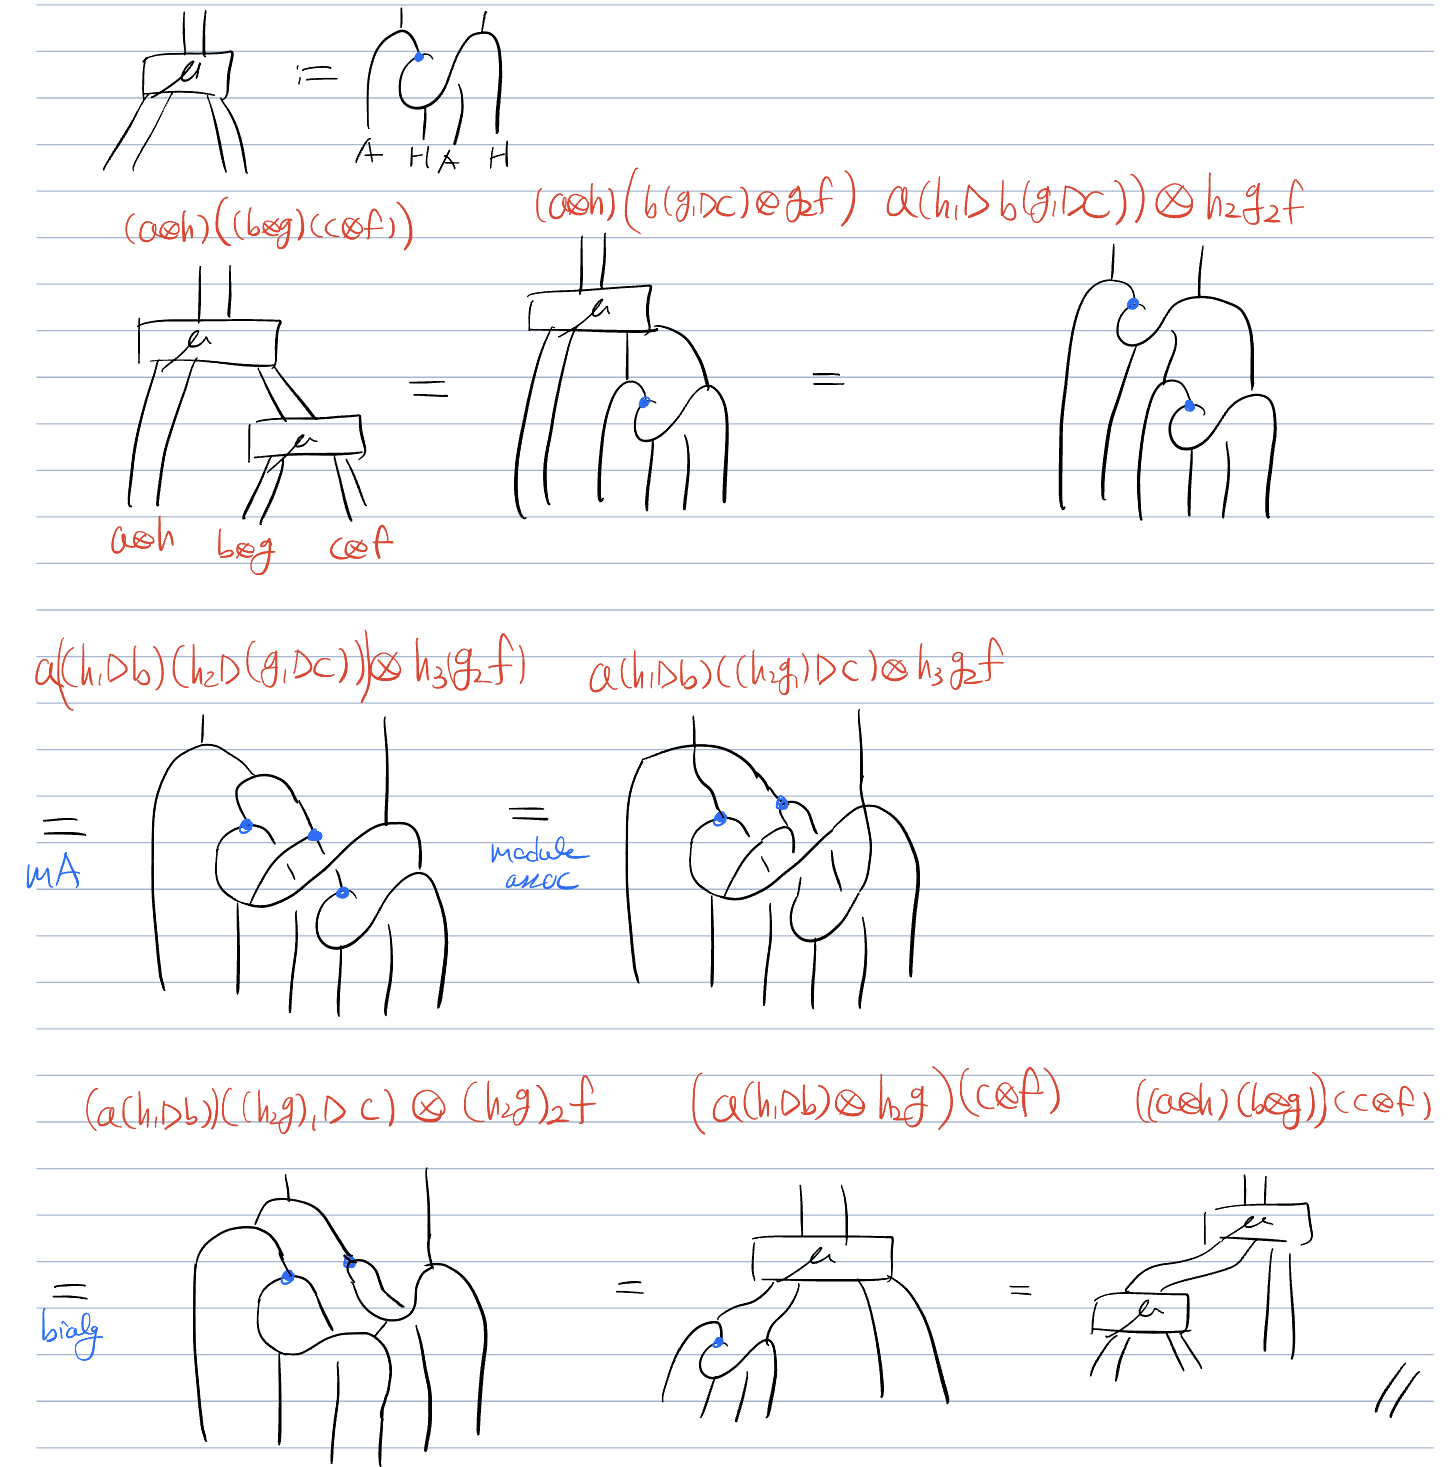
\includegraphics[width=\linewidth]{attachments/260906_pf_Prop1.6.6.png}
        \par\nobreak\smallskip
        \hfill\qedhere
    \end{minipage}
\end{proof}

Its comodule coalgebra version is described as follows.


